\documentclass{article}
\usepackage[utf8]{inputenc}
\usepackage[letterpaper,margin=1in]{geometry}
\usepackage{graphicx}
 
\title{\bf{ Lab4: Real-Time Operating Systems} }

\author{Group 2: Shi Su \& Mengjin Yan}
\date{December 2, 2015}
 
\renewcommand*\contentsname{Content}
 
\begin{document}
 
\maketitle
 
\tableofcontents

\newpage

%%%%%%%%%%%
% OVERVIEW
%%%%%%%%%%%

%\section{Overview}
% 
%On the basis of lab2 to implement a small kernel - {\bf Gravel}, adding the IRQ handling and timer driver.\\
%\newline
%\begin{figure}[h]
%\centering
% 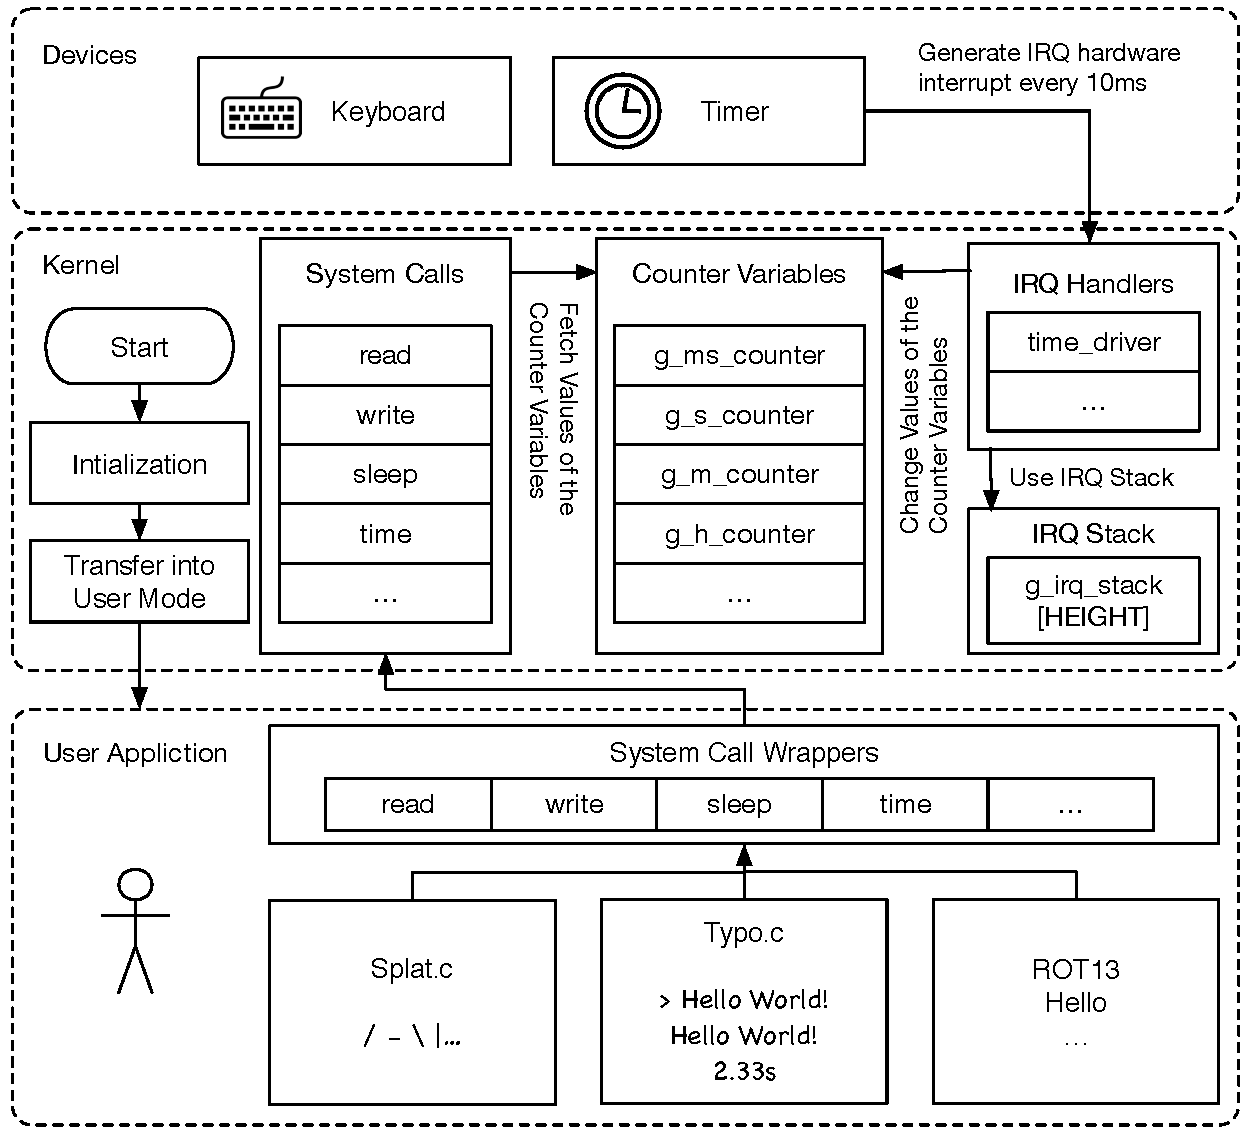
\includegraphics[scale=0.8]{workflow.pdf}\\
% \caption{Modules of Gravel}
% \end{figure}
  
%\newpage

%\section{Workflow}
\section{Kernel Initiation}
\begin{itemize}
	\setlength{\itemsep}{1pt}
	\setlength{\parskip}{0pt}
	\setlength{\parsep}{0pt}
	\item Store the value of r8 (uboot function table) to global variable {\it global\_data}
	\item Wire in SWI/IRQ handler
	\item Set up IRQ stack\\
		A chuck of memory is allocated for IRQ stack in data section as the global variable array {\it g\_irq\_stack}, we don't need to specified its location explicitly and worry about it will be clobbered by code or stack. Since array grows from lower address to higher address, while the growth direction of stack is opposite. So sp is set to point at the highest address(end) of array {\it g\_irq\_stack}. 
	\smallskip
	\item Initiate interrupt controller\\
		Update ICMR to mask interrupt from all interrupt except OSMR0.\\
		Update ICLR to route interrupt from OSMR0 as IRQ.
		\smallskip
	\item initiate Mutex
		Update global variable {\it gtMutex}, set all mutex as available
		\smallskip
	\item Initiate Timer
		Set all time counter variables to 0.\\
		Set the value of OSSR to 0\\
		Update OIER to enable the interrupt from OSMR0\\
		Set the value of OSMR0 to 32500, which corresponds to 10ms resolution\\
\end{itemize}

%%%%%%%%%%%
% Task creation
%%%%%%%%%%%
\section{Task Creation}
\begin{itemize}
	\setlength{\itemsep}{1pt}
	\setlength{\parskip}{0pt}
	\setlength{\parsep}{0pt}
	\item test
\end{itemize}

%%%%%%%%%%%
% Context Switch
%%%%%%%%%%%
\section{Context Switch}
When an IRQ interrupt is generated, the system automatically changes into IQR mode and the interrupt is handled by the IRQ handler which is consist of two parts, irq\_handler.S and c\_irq\_handler.c.\\
In irq\_handler.S:
	 \begin{itemize}
	  \setlength{\itemsep}{1pt}
	  \setlength{\parskip}{0pt}
	  \setlength{\parsep}{0pt}
	\item Store non-banked user/supervisor mode register on stack
	\item Branch into c\_swi\_handler
	\end{itemize}
In c\_irq\_handler.c:
	\begin{itemize}
	  \setlength{\itemsep}{1pt}
	  \setlength{\parskip}{0pt}
	  \setlength{\parsep}{0pt}
	\item Read the value of ICMR to determine which device generated the IRQ 
	\item Branch to corresponding ISR
\end{itemize}

%%%%%%%%%%%
% Event wait
%%%%%%%%%%%
\subsection{Event Wait}	
One sentence

 \begin{itemize}
	  \setlength{\itemsep}{1pt}
	  \setlength{\parskip}{0pt}
	  \setlength{\parsep}{0pt}
	  \item test
\end{itemize}

%%%%%%%%%%%
% Dev update
%%%%%%%%%%%
\subsection{Device Update}	
One sentence
 \begin{itemize}
	  \setlength{\itemsep}{1pt}
	  \setlength{\parskip}{0pt}
	  \setlength{\parsep}{0pt}
	  \item test
\end{itemize}

%%%%%%%%%%%
% Mutex
%%%%%%%%%%%
\subsection{Mutex Lock \& Unlock}	
One sentence
 \begin{itemize}
	  \setlength{\itemsep}{1pt}
	  \setlength{\parskip}{0pt}
	  \setlength{\parsep}{0pt}
	  \item test
\end{itemize}


%%%%%%%%%%%
% New System Calls
%%%%%%%%%%%	
\section{New System Calls}
\begin{itemize}
\item{task\_create}\\
	int task\_create(task\_t* tasks, size\_t num\_tasks)\\
	\newline
	{}

\item{mutex\_create}\\
	int mutex\_create(void)\\
	\newline
	{}

\item{mutex\_lock}\\
	int mutex\_lock(int mutex);\\
	\newline
	{}

\item{mutex\_unlock}\\
	int mutex\_unlock(int mutex);\\
	\newline
	{}

\item{event\_wait}\\
	int event\_wait(unsigned int dev);\\
	\newline
	{}
\end{itemize}


	
 
\end{document}